\newcommand{\FigureHighMeasure}{
\begin{figure}[t]
    \centering
    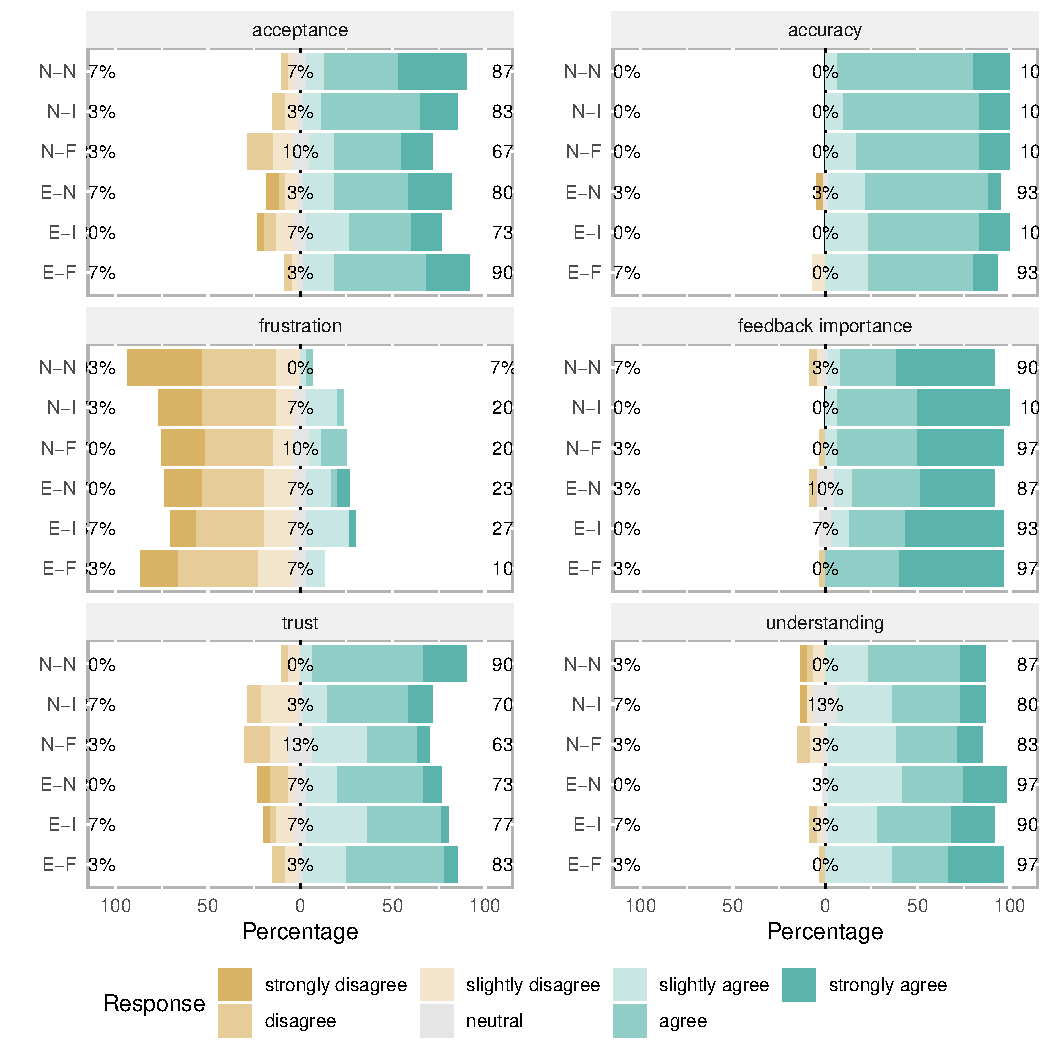
\includegraphics[width=.48\textwidth]{2020_chi_explanation/figures/study2-measures.pdf}
    \caption{Study 2 responses by condition for the main subjective measures (except expected change). Participants were more satisfied, but trust suggests nuance (e.g., E-N vs. N-N, without feedback, explanation has a negative impact).
    %on seven-point  scales from ``strongly disagree'' to ``strongly agree.'' 
    (Figure~\ref{fig:study1measures} describes $y$-axis labels.)}
    \label{fig:study2measures}
    \vspace{-10pt}
\end{figure}
}

\newcommand{\FigureHighExp}{
\begin{figure}[t]
    \centering
    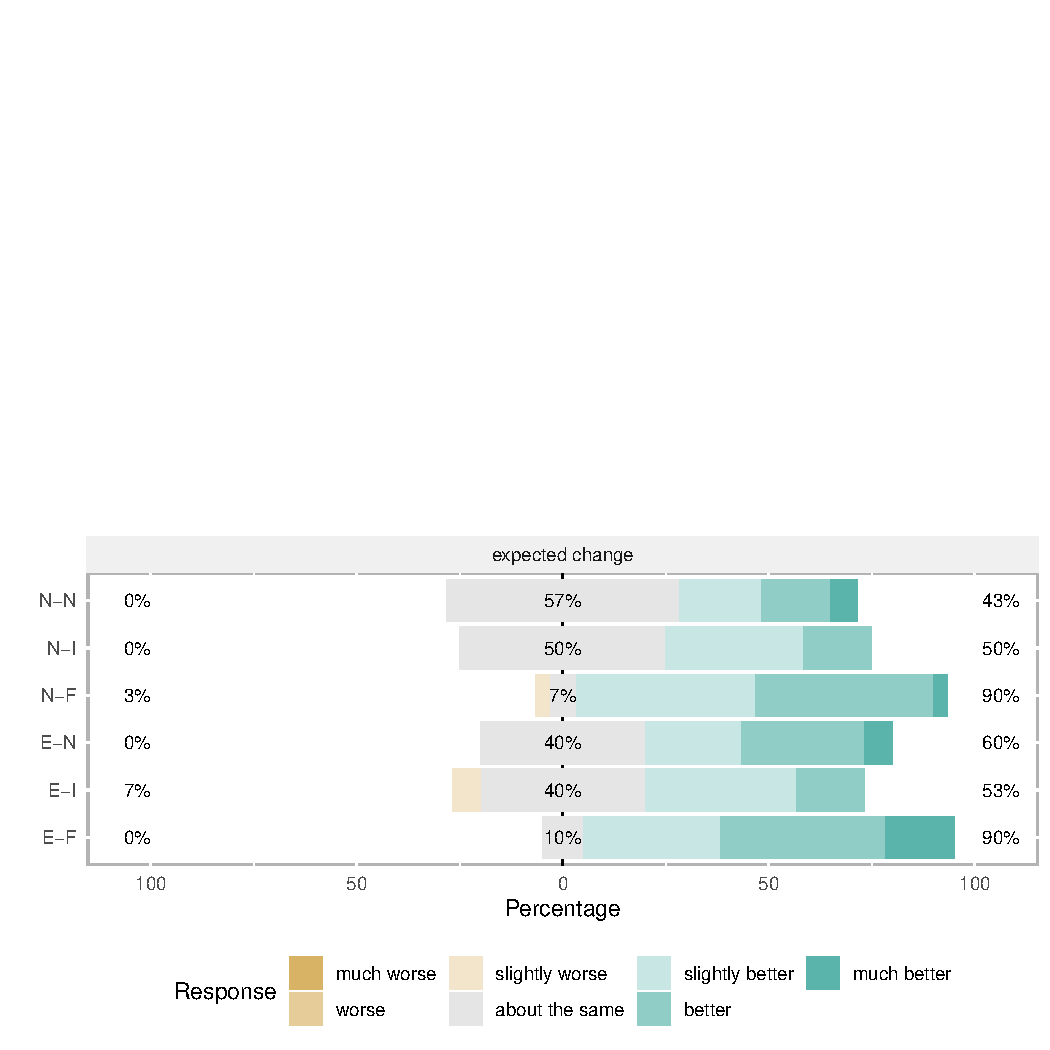
\includegraphics[width=.48\textwidth]{2020_chi_explanation/figures/exp-plots-study2.pdf}
    \caption{Study 2 responses for the expected change measure by condition, showing that in general participants expected improvements (green bars), but more in feature-level feedback conditions (E-F and N-F). (See Figure~\ref{fig:study1measures} for a description of y-axis labels).}
    \label{fig:study2exp}
    \vspace{-10pt}
\end{figure}
}